\chapter{Industrial context and research framework} \label{Industrial Context and Research Framework}
\minitoc

In this first chapter, we present the industrial context of this research project. Primarily, we will review the Industry 4.0 paradigm as well as the benefits it can bring to the manufacturing industry through the application of Machine Learning methods. Subsequently, we will describe our extrusion blow-moulding industrial research framework, and we will formalise and position our research work. Finally, the goal of this research work is presented: the quality improvement of fuel tank production using extrusion blow-moulding process.  

\section{Industry 4.0: a promise for improved manufacturing}

Automotive industry is nowadays driven by global competition and the need for fast adaptation of production to the ever-changing market requests. The fourth revolution in industry, Industry 4.0, holds the promise of increased flexibility in manufacturing, along with mass customisation, better quality, and improved productivity \citep{zhong2017intelligent}. As already occurred for the past three revolutions, technical innovations and a new way of perceiving the world, are radically changing the industry. The first industrial revolution at the end of the 18th century introduced steam-powered machines. The second one used electricity to improve productivity and to create mass production. Electronics and information technology, with the introduction of Programmable Logic Controllers (PLC) began the industrial automation and the third industrial revolution. The context of billions of people connected by mobile devices, with unprecedented processing power, storage capacity, and access to knowledge is promoting the emergence of new technologies. Artificial intelligence, robotics, autonomous vehicles, 3-D printing, nanotechnology, biotechnology, materials science, energy storage, and quantum computing are changing the world and today we are on the cusp of the fourth industrial revolution \citep{schwab20164th}.  

The term Industry 4.0 refers to the connection among production departments, tools, machines, “individual things” in general made possible by internet and cyber physical systems \citep{schlapfer2015industry}.
With the digital revolution, the boundaries between physical and digital worlds are disappearing to create an interconnected factory with strong interactions between employees, machines and products. These connected entities can interact with one another using standard internet-based protocols and analyse data to predict failure, configure themselves, and adapt themselves to changes.
According to the estimations made by BCG for German companies, Industry 4.0 will have a positive impact on companies with productivity and revenue growth but also on economy with more investments and with an overall six percent increase in employment during the next ten years. Productivity improvements on conversion costs, which exclude the cost of materials, will range from 10 to 20\% in automotive industry, while productivity gains of 5 to 8\% will be achieved if the materials costs are factored in \citep{lorenz2016time}. The revenue growth, as a direct consequence of  manufacturers' demand for enhanced equipment and new data applications, as well as consumer demand for a wider variety of increasingly customised products, is estimated at 30 billion euros a year, which is approximately one percent of the German GDP \citep{russmann2015industry}. 

Industry 4.0 is also a new way of looking at performance, with a more precise and immediate vision (based on real-time indicators) of the entire production chain, but also the optimisation of production through the use of artificial intelligence. In interconnected plants, the large amount of data collected from different sources --production equipment and systems as well as enterprise-- can be helpful in taking decision and contributes to a continuous improvement process. In particular, we think that the integration of machine learning models inside complex industrial processes can reduce the non-quality costs with the increase of the Overall Equipment Effectiveness (OEE). 

In the following, we will present what we consider to be the two key elements that have been contributing most to the fourth industrial revolution: data and machine learning.


\subsection{Data}

For a long time, information was documented on paper while manufacturing was realised by handicraft, therefore, the integration between information technology and manufacturing technology was neither beneficial nor feasible. Since the advent of the first electronic computer in 1940s, the rapid development of information technology (IT) has been driving manufacturing toward informatisation. Since the 1960s, the development of integrated circuits has paved the way for the advancement of computer hardware and software. Since the 1980s, TCP/IP, local area networks (LAN), the World Wide Web (WWW), and search engines emerged one after another to meet the increasing needs for data storage, indexing, processing and exchange. All these information technologies were widely applied in manufacturing. As a result, many advanced manufacturing technologies were put forward, such as computer integrated manufacturing (CIM), computer aided design (CAD), manufacturing execution system (MES), computer aided manufacturing (CAM), enterprise resource planning (ERP), and networked manufacturing (NM), etc. Recently, the rise of New IT technologies such us IoT (Internet of Things) and cloud solutions provides new sources of data. Due to the deep fusion between IT and manufacturing on going, the degree of manufacturing smartness is progressively elevating. As a result, manufacturing data also becomes increasingly richer \citep{tao2018data}.

As a consequence of the multitude of manufacturing technologies, industrial data comes in very different forms. This implies a lot of heterogeneity in the data which tends to make it harder any data usage or comparison. Moreover, most of data available in manufacturing industry is \textit{unstructured}. In this thesis we consider as \textit{structured} any kind of data that can be stored in form of rows and columns in systems like databases or Excel spreadsheet. Any data that can be stored by respecting this convention, without loosing any information, will be qualified as a structured data. On the other hand, we qualify as \textit{unstructured} any set of data that cannot be stored in a set of rows and columns without loosing information. Some types of data may be difficult to definitely classify into one or the other category. It can actually depend on the use-case and the data processing objective. For example, an image can be represented as a 2D matrix (for black and white images) or as 3D matrix (for colour images). This representation is perfectly structured. Therefore an image, or a video, can be considered as a structured data format for someone willing to conduct a spectral analysis, only interested in the pixel values and positions. Nonetheless, the same image can also be considered unstructured if we focus our interest on the content of the image. Indeed, pixel values can not be easily translated into a structured representation of the actual content.

Unfortunately, dealing with unstructured data is much more challenging in a data science perspective \citep{blumberg2003problem,sagiroglu2013big,buneman1997adding}. It requires highly complex, expensive and time-consuming feature extraction processes and operations (i.e. a feature represents a descriptor (e.g. colour of a car) in a data science context). It is estimated that the average \textit{Information Systems} (IS) roughly contain around 15\% of structured data and 85\% of unstructured data. Such an assumption seems consistent with the actual status of the manufacturing industry. Furthermore, even if a more optimistic situation is considered, with a balanced rate of 50\% structured and 50\% unstructured data, it still appears critical to be able to mine, explore, exploit, and search this data. Consequently, we could argue that a big data context is inherently linked to unstructured data.
Dealing with manufacturing data implies to use and manage large amounts of human-made data. This data comes with inherent and recurring issues which highly limit its usability without an extensive pre-processing.

\subsection{Machine learning and deep learning}

As highlighted in the previous section, the amount of available data is exponentially increasing and it can be reasonably considered that humans will not be able, in a near future, to process, by hand, these massive amounts of data any more and perform heavy computations in a parallel manner. Nonetheless, machine learning and deep-learning (see Section \ref{Machine learning and Deep Learning}) take advantage of parallel computation capabilities and large data quantities to approach human behaviours and understanding in complex situations. Machine learning, and more generally data-driven methods, provide a new way to deal with manufacturing problems. 

In the last decade, the hottest machine learning sub-field, deep learning, has gained a lot of popularity due to its ability to provide state-of-the-art results in multiple domains. Deep learning is not a new idea, most of the recent proposed deep learning architectures rely on advances from the last decades of the 20th century. Deep learning regained attention when \citet{krizhevsky2012imagenet} outperformed by a large margin all the other teams on the ImageNet \citep{deng2009imagenet} image classification task using a deep convolutional neural network. The reborn popularity of these computational methods can be attributed to the following reasons:

\begin{itemize}
    \item \emph{Increasing computer power}: GPU (Graphical Processing Unit) computing enabled, in the early 2010s, improved calculation performance in the field of machine learning. Powerful, fast and cheap GPU-devices greatly helped researchers to reach performances never achieved before. Deep learning involves huge amount of matrix multiplications and other operations which can be massively parallelised and thus sped up on GPUs.
    \item \emph{Larger labeled datasets}: the advent of big data has considerably increased the size of the datasets available in manufacturing companies. The availability of an important amount of data is indispensable for the successful application of deep learning methods that require, in average, more data compared to conventional machine learning approaches. For instance, the ImageNet dataset \citep{deng2009imagenet} released in 2009, contains more than 14 millions annotated images that can be used for training image classifiers.
    \item \emph{Advances in deep learning research}: deep learning is one of the most popular research topics of the moment and interest in this area is growing every year. As pointed by the ``AI index 2019 report''  \citep{zhang2021ai}, between 1998 and 2018, the volume of peer-reviewed AI papers has grown by more than 300\%, accounting for 3\% of peer-reviewed journal (Figure \ref{fig:Number of Peer-Reviewed AI Publications}) publications and 9\% of published conference papers. This increase in the number of researchers leads to faster research progression. 
    \item \emph{Open source tools and models}: the democratisation of open sources frameworks such as \textit{PyTorch} \citep{paszke2019pytorch}, \textit{Tensorflow} \citep{tensorflow2015-whitepaper}, \textit{Keras} \citep{chollet2015keras} and \textit{Scikit-Learn} \citep{scikit-learn} allow to apply machine learning and deep learning methods with a few line of code. Moreover, the machine learning community is rather open in sharing results. There are many pre-trained models available online, ready to be used as a starting point for \textit{transfer learning} (\ref{Transfer Learning}).  
\end{itemize}

\begin{figure}
\centerline{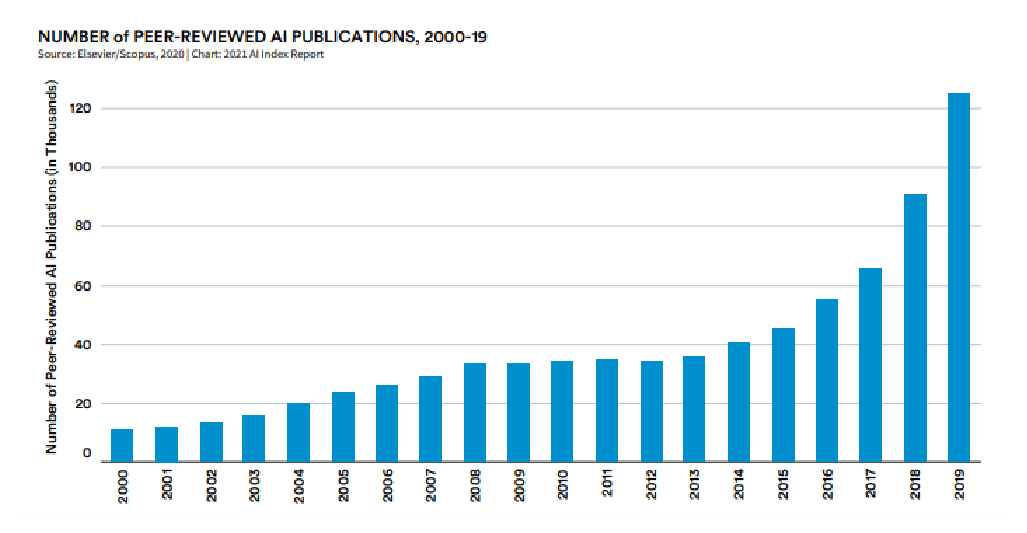
\includegraphics[scale=0.9]{images/chapter_1/AI_report.eps}}
\caption{Number of peer-reviewed AI publications, 2000-2019 \citep{zhang2021ai}}
\label{fig:Number of Peer-Reviewed AI Publications}
\end{figure}


\subsection{Review of opportunities for the manufacturing industry}

In this section, we present the result of a literature review we conducted to highlight some of the possible applications where machine learning could be applied in order to create value for manufacturing companies. This study should not, in any case, be considered as an exhaustive list of possibilities. Results are summarised in Table \ref{tab:ai_benefits}. 

\begin{table}
\label{tab:ai_benefits}
\caption{ML opportunities in manufacturing}
\begin{tabular}{|l|p{6cm}|p{4cm}|}
\hline
%
Domain &
  Benefits &
    Bibliography \\ \hline
Quality  &
  Decrease the product failure rate at the end of the production line. Optimise key performance index of the final product to meet customer needs. &
    \citep{lieber2013quality, li2018ensemble, chen2008neural, nagorny2017quality, haeussler1996quality} \\ \hline

Maintenance &
  Increase the availability of the production line by preventing the breakdown of equipment in advance. Predict the risk of malfunction of the production line and arrange proactive maintenance. &
    \citep{nguyen2019new, lee2017application, einabadi2019dynamic, li2017intelligent, liu2016prediction}\\ \hline
Fault Diagnosis &
  Prognostic diagnose of production line failure event. Identify the malfunction device of the production line. Predict the abnormal behaviours of machines and equipments. & \citep{toma2020bearing, wong2006modified, chen2014fault, malik2017artificial, arabaci2010automatic} \\ \hline
Scheduling  &
  Logistic management of the production line, which can maximise the throughput of the production line. Buffer control and product routing management. & \citep{morariu2020machine, woschank2020review, lolli2019machine, zhang2019review, gomes2016developing} \\ \hline
\end{tabular}
\end{table}


\section{Industrial domain: extrusion blow-moulding} \label{Industrial domain: extrusion blow-moulding}

Our industrial process, extrusion blow-moulding, is used to form hollow thermoplastic objects (especially bottles and containers). The process takes a thin-walled tube called a \textit{parison} that has been formed by extrusion, entraps it between two halves of a larger diameter mould, and then expands it by blowing air into the tube, forcing the parison out against the mould. The outside of the thin-walled part takes then the shape of the inside of the mould \citep{poli2001design}.

\begin{figure}
\centerline{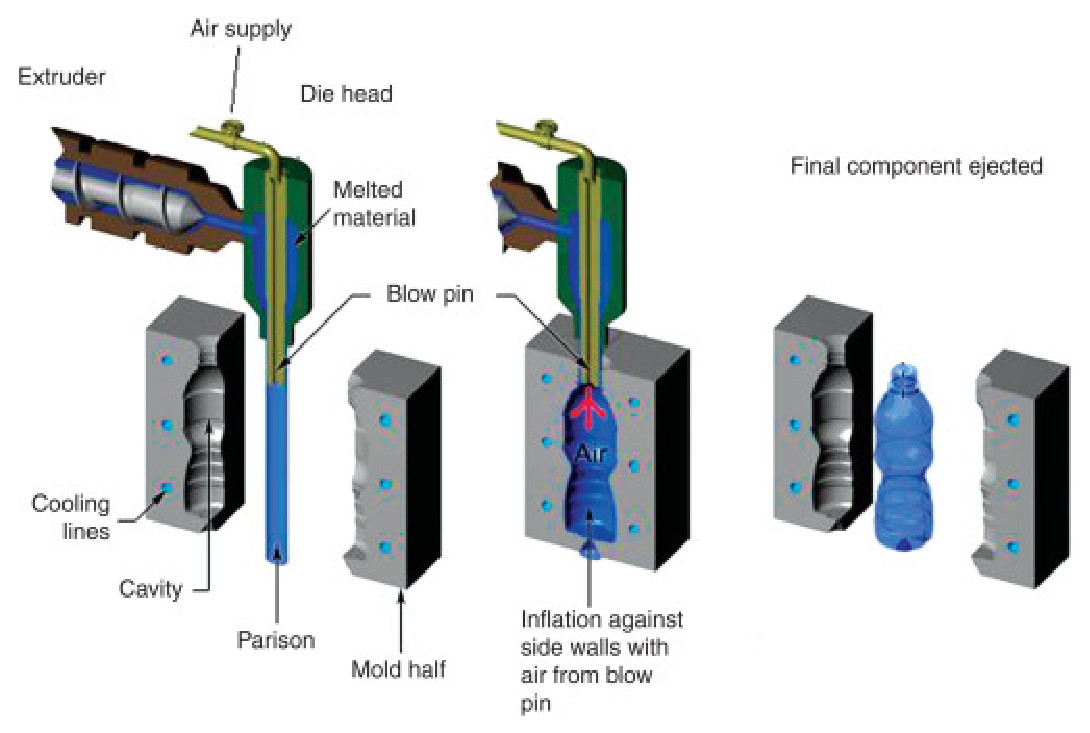
\includegraphics[scale=0.75]{images/chapter_1/extrusion_blow_molding.eps}}
\caption{Extrusion blow-moulding \citep{goodship2015design}}
\label{fig:Extrusion Blow-moulding}
\end{figure}

As the name suggests, extrusion blow-moulding is composed of two sub-processes: extrusion and blow-moulding.

\begin{itemize}
    \item \textit{Extrusion:} extrusion is a continuous-flow process where a plastic material feedstock is fed through a hopper onto a feeding transfer screw. The thermal energy provided by the heating clamps as well as the mechanical energy provided by the screw rotation allows the melting of the plastic material.The melted material is then pushed into an extrusion head and the die gap will typically create a tubular extruded cross-section, round or oval depending upon the final shape of the finished blow moulded part.
    The die gap is the distance between the inner mandrel and the outer bushing. The gap can be varied during the extrusion, due to the tapered nature of the die, by moving either the mandrel or the bushing in a vertical direction. The process of variable die gap extrusion is referred to as parison programming and is utilised to manipulate the thickness distribution in the final part \citep{diraddo1993profile}.
    \item \textit{Blow-moulding:} Unlike extrusion, blow-moulding is a discontinuous-flow process. In extrusion blow moulding, the parison is vertically suspended in the air during which time two mould halves enclose it by the action of a pneumatic or hydraulic mechanism. Internally applied air pressure causes the parison to inflate and take the shape of the inner parts of the moulds. Once the blow operation is completed and the part has been cooled down suitably for ejection, the mould opens and the part is ejected, allowing the parison to be extruded through the mould for the next cycle. 
\end{itemize}

Each phase has parameters that influence the subsequent phases and, ultimately, the characteristics of the finished product. The multiple phases mean that the number of parameters that can be adjusted on the process is fairly high. It is possible to fine-tune temperatures, screw speeds and throughputs for the extrusion, as well as the  pressure curves, moulds opening and closing times for the blow-moulding phase. In addition, the extrusion blow-moulding process has a certain dynamic: it takes a certain amount of time for the adjustment of one of the process parameters to have an effect on the products. This dynamic is mainly due to the thermal inertia of the solid tooling.
One of the most critical part of the process is the parison formation. In fact, the dimensions of the blow moulded article are directly related to the dimension and thickness of the parison. Furthermore, the thermo-mechanical history of the material during the parison formation stage and the resulting weight and diameter distribution of the parison have a great influence on the characteristics of the subsequent inflation and cooling stages. The shape and the dimensions of the parison are the result of complex interactions between the molten polymer and the thermo-mechanical conditions that influence the melt after it leaves the extruder die. Parison formation is affected by two phenomena knows as \textit{swell} and \textit{sag}. Parison swell, occurring both in diameter and thickness, is due to the nonlinear viscoelastic deformation of the polymer melt in the extrusion die. Sag is caused by gravitational forces that act on the suspended parison \citep{huang2002prediction}.

There are many variations of this process including equipment made to extrude multiple parisons simultaneously, equipment that can extrude multiple layers within the same parison, equipment with rotary capability that will hold several moulds and can provide a continuous nonstop process. Moreover, the extrusion blow-moulding process can be split into two subcategories: intermittent extrusion blow moulding and continuous extrusion blow moulding. With intermittent extrusion blow moulding, the extruder fills a reservoir with plastic. Once the reservoir has been filled, a plunger is activated and pushes the material from the reservoir through the extrusion head. On the other hand, in continuous blow-moulding, the plastic is extruded permanently in a continuous manner while the machine runs.

In this thesis project we have been studying a continuous extrusion blow-moulding process, whose finished products are obtained from the overlay of multiple plastic layers. This particular type of blow-moulding process is known as \textit{co-extrusion}. Co-extrusion was born out of the need of reduce the permeability of fuel tanks. The steps for producing a multi-layer plastic product are the same as those used by the traditional single layer process, except for the number of extruders involved in the manufacturing process. Up to six extruders can be used simultaneously to melt different plastic materials. The goal is to create a multi-layer tank with the use of different materials, as shown in Figure \ref{fig:Co-extrusion Process}.

\begin{figure}
\centerline{\includegraphics[scale=0.55]{images/chapter_1/coextrusion.png}}
\caption{Co-extrusion process}
\label{fig:Co-extrusion Process}
\end{figure}

The extrusion blow-molding process taken into account all along this research study is used to produce different tank models. In fact, by simply changing the moulds, it is possible to manufacture tanks with various shapes and sizes. The ratio between the separate plastic layers, as well as the material throughput, need to be adjusted accordingly to take into account the different size or shape of each tank model. This makes the extrusion blow-molding a flexible process which allows for rapid responses to costumers requests. The fuel tanks are usually manufactured in production campaigns of a few days, also known as batches.

The extrusion blow-moulding constitutes one of the various stages necessary to produce finished part. The stages needed to manufacture a finished part may vary depending on the type of product. For instance, a fuel tank container, a plastic bottle or a plastic bumper may require different post-production processes. Further information on how a fuel tank is produced are available in Appendix \ref{Fuel system production process}. As far as our thesis work is concerned, we will only focus on the extrusion blow-moulding stage.

\subsection{The key parameters of extrusion blow-moulding} \label{The key parameters of the Extrusion Blow-moulding}

Extrusion blow-moulding requires the fine-tuning of multiples adjustable parameters to reach the conditions for producing the final part. One of the most critical process parameter involving the extrusion sub-process is the material throughput. Controlling the amount of material passing through each extruder is crucial for the following reasons:  
%
\begin{itemize}
    \item It affects the cycle time. The throughput affects the ejection rate of the parison and therefore the cycle time. A cycle time reduction results in an higher manufacturing rate.
    \item The throughput ratios among the different 6 extruders should be controlled to ensure the correct amount of material on each of the 6 layers composing the tank thickness.
\end{itemize}
%
The throughput depends mainly on the rotation speed of the extruder and slightly on the extruder temperature. The temperature of the extruder affects the melting of the plastic material and the material viscosity may change. Depending on the material viscosity the throughput may change given the same extruder speed. For what has been said so far, controlling the temperature of the extruder along the screw length is mandatory to ensure constant and repeatable melting condition and therefore ensure a constant throughput. Another key parameter is the opening of the die gap of the \textit{head} of the machine. By controlling the opening of the gap during the cycle time we are able to distribute more or less material along the parison length. This operation is important to ensure to put enough material in parison zones that are most stretched during the blowing phase. Of course, the parison length plays a key role in ensuring that the material distribution is well positioned relatively to the mould position. Unfortunately, in the production process in question, there is no control system for measuring the parison length. In continuous extrusion blow-moulding, the cycle time triggers the blowing cycle. 

\begin{landscape}
\begin{table}
\caption{Blow-moulding key
parameters}
\label{tab:key_parameters}
\begin{small}
\begin{tabular}{@{}llll@{}}
\toprule
\multicolumn{4}{c}{\textbf{Extrusion}} \\
\midrule
\textbf{Parameter}                     & \textbf{Range}   & \textbf{Description}                                    & \textbf{Dependencies} \\ 
\midrule
Speed$^*$  (in RPM)                                  & [0, 90]       & Rotation speed of the screw                               &              \\ 
Throughput$^*$ (in Kg/h)                             & [0, 400]      & Material throughput in screw                 &  Speed, temperatures            \\ 
Melt pressure$^*$ (in \% of motor nominal torque)    & [0, 100]      & Pressure at the end of the screw                 & Speed             \\
Feeding temperature$^*$ (in \degree C)                      & [0, 100]      & Temperature at the entrance      &              \\
Melt temperature$^*$  (in \degree C)                        & [0, 250]      & Temperature at the end          &    Feed. temperature, pressure          \\
Cycle time   (in s)                                  & [60, 120]     & Tank production cycle time                                &              \\
Parison profile  (in \%)          &  [0, 100]     &  Die gap opening                                              &  Cycle time            \\
Parison length (in mm)                               & [0, 3000]     & Length during extrusion     &   Parison profile, cycle time    \\ 
\midrule
\multicolumn{4}{c}{\textbf{Blow-moulding}} \\
\midrule
\textbf{Parameter}                     & \textbf{Range}   & \textbf{Description}    & \textbf{Dependencies} \\ 
\midrule
Blowing pressure$^{**}$ (in bar)      &  [0, 12]              & Blowing pressure inside moulds                                               &              \\
Cooling water temperature (in \degree C)     &  [5, 30]               & Temperature of cooling water (moulds)                                               &               \\
\bottomrule
\end{tabular}
\end{small}

\footnotesize{%
\noindent
$^*$ For each extruder \\
\noindent
$^{**}$ There exist 4 different blowing circuits}\\
\end{table}
\end{landscape}

With regard to the blow-moulding sub-process, the most critical parameters are the blowing pressure pressures (there exist 4 different air blowing circuits), the cooling water temperature and its throughput. The blowing pressure ensures the parison to inflate and take the shape of the inner parts of the moulds. Without enough air pressure the plastic material does not adhere to the mould surfaces, preventing a correct material cooling. In the same way, the amount of water passing through the cooling circuit, as well as its temperature, affect the cooling capacities of the moulds. Table \ref{tab:key_parameters} summarises the key parameters of an extrusion blow-moulding process that were identified together with process experts.

\subsection{The key quality characteristics of a blow-moulded fuel tank} \label{The key quality characteristics of a blow-moulded fuel tank}

Quality control is generally expressed as  the verification of the conformity of the process and the product/service to the requirements of its quality standard. The ISO 9000 standard defines quality control as ``a part of quality management focused on fulfilling quality requirements'' \citep{iso9000}. In our context, the requirements are defined by the customers, and measurements on the product and compared with the customer requirements, if the measurements meet the customer specifications, the part can be sent to the customer, otherwise the part must be rejected. In blow-moulded parts, , the distribution of the material over the entire surface of the part surface plays a key role in ensuring that the finished product meets customer specifications. In the extrusion blow-moulding process, we are mostly interested in the dimensional/geometric characteristics. In fact, the main purpose of the quality control of the blow-moulded part is to asses the integrity of the plastic shell. The thickness of the tank over the whole surface must be sufficient to ensure the robustness of the part and therefore its safety, while avoiding unnecessary excess weight on the finished product. Measuring the thickness of a hollow blow-moulded part is difficult as there is no access to the inner surface. Moreover, the thickness is relatively small, with value ranging from $3$ to $8$ millimetres. This requires an indirect measurement with an accuracy of at least $0.1$ millimetres.

\paragraph{Background in thickness measurement}

Traditional methods to measure the thickness of hollow parts rely on ultrasonic instruments that provide satisfactory results while avoiding the destruction of parts. The principle of \textit{Ultrasonic Thickness Measurement} (UTM) is to measure the time needed for the ultrasonic wave to traverse the material. Some of the advantages of UTM over other nondestructive methods are:
\begin{itemize}
    \item the possibility to measure parts with just one accessible surface,
    \item the suitability to industrial conditions,
    \item its sensitivity and accuracy.
\end{itemize}
 
These methods are extremely accurate for sample quality control, but they present a major drawback: they cannot be used for online measurement. The measurement of a large number of points, which is necessary to estimate the distribution of the material over the entire surface, is time-consuming and cannot be done online in production. Hence, the quality control of wall thickness is only carried using a sampling approach. Recently, new technologies involving the use of terahertz waves have been developed to accurately measure the thickness of materials without any contact with the material itself. These methods have proven to be extremely powerful for measuring the thickness of automobile paint \citep{su2014terahertz,krimi2016highly}, or pharmaceutical tablets \citep{may2011terahertz}. Of all the methods found in the literature, terahertz-based systems seem to be the only ones that can be used to perform real-time thickness measurement, but in order to use them in real-time, the measurement sensor must be installed on a robot, or collaborative robot, which can significantly affect the price of the complete measurement solution.

Another well-known technique for measuring thickness of parts is \textit{Computed Tomography} (CT). Typical areas of use for CT in industry are in the detection of flaws such as voids and cracks, and particle analysis in materials. In metrology, CT allows measurements of the external as well as the internal geometry of complex parts. As stated by \citet{de2014industrial}, CT is particularly suitable to investigate moulded polymer parts, thanks to the good penetrability of X-rays in this material. Even if CT-based techniques are extremely powerful, they require laboratory conditions and  do not lend themselves well to real-time thickness control. Moreover, this equipment may be very expensive, questioning its profitability.
%
Eddy current testing, widely applied for the non-destructive thickness measurement of metallic parts \citep{cheng2017thickness,mao2016thickness,wang2015noncontact,yin2007thickness}  is also non-destructive, but cannot be used as polymers composing the blow-moulded part are not conductive.

In the last decades,\textit{thermal imaging}, a non-contact technology capable of measuring large surfaces in a single shot, has been studied as a possible method to infer the thickness of a solid element \citep{sun2003method,sun2006analysis,choi2008quantitative,benitez2008definition,zeng2012absolute,li2018thickness,he2013eddy}. Among the most widely used thermal imaging approaches we can mention: \textit{pulsed thermography} in which a brief controlled thermal stimulation pulse is applied on the tested piece, \textit{step heating thermography}, in which a continuous, uniform heat flow is applied for a long period, and \textit{lockin thermography}, in which a periodic heat input is used. The main idea behind these approaches is to transfer energy to the test piece and to monitor its surface temperature evolution over time. In flash thermal imaging, for example, some flash lamps provide the thermal impulse, and the infrared camera monitors the surface-temperature decay on the heated surface. On the other hand, step-heating thermal imaging is using a long pulse of low intensity heat stimulation. Unlike pulsed thermal imaging, step-heating technology monitors the temperature raise over time while the heat energy is transferred to the test piece. The approach of monitoring the surface-temperature may also be applied without actively providing heat to the test part, especially for parts that are hot after the manufacturing process. The proposition of thermal imaging to measure the thickness of the tank is one of the major contributions of this research work and the proposed approach will be presented in detail in Chapter~\ref{Thickness inference using thermal imaging}.

Due to the impossibility of measuring the thickness of all parts produced, in practice, weight is often measured as an alternative. The weight is an indicator of how much material is composing the part and allows for an overall control of the quality of the part. The weight has a lower boundary to ensure that sufficient material is composing the tank and an upper boundary to avoid unnecessary weight of the finished product. Unlike the thickness, which has to be measured in several areas of the tank and cannot be carried out online for all the parts, the weight requires a simple weight scale, placed in the area where the blow-moulded part is discharged. 

Another quality issue that may occur is the fuel tank contamination. If the extrusion blow-moulding machine screws are not properly emptied following the so called purge procedures, or cycles, some material can remain attached to the screws and can solidify. This may cause the presence of unwanted burned material in the manufactured fuel tank, which generates a visual non-conformity of the part, and which can lead to tank permeability problems. The contamination problem identification completely relies on human visual inspection.

In order to produce a complete fuel system (see Appendix \ref{Plastic Omnium}), other manufacturing process are required after the extrusion blow-moulding (see Appendix \ref{Fuel system production process}). Operations such as components welding or the assembly of pieces require further quality checks. The deepening of any quality control that does not directly concern the extrusion blow-moulding is out of the scope of this research work.  
%
\begin{table}
\caption{Quality indicators of a blow-moulded fuel tank }
\label{tab:quality_inidcators}
\begin{tabular}{@{}lllp{6cm}@{}}
\toprule
\textbf{Indicator} & \textbf{Unit} & \textbf{Value range} & \textbf{Description}                                                 \\ 
\midrule
Global Thickness           & mm                        & {[}3, 8{]}           & Thickness of the part measured at several critical points \\ 
Weight & Kg & {[}6, 14{]} & Total weight \\ 
\bottomrule
\end{tabular}
\end{table}
%
Table \ref{tab:quality_inidcators} summarises the two quality characteristics of a blow-moulded part we are interested in, and which must be monitored to ensure that the parts produced comply with customer requirements. However, in Chapter \ref{From Corrective to Predictive Process Control}, we will present an initiative which aims to partially reduce the contamination problems.

\section{Quality control and process monitoring in the extrusion blow-moulding process: a state-of-the-art} \label{state-of-the-art}

A literature review was carried out to identify previous work aimed at improving the overall quality of parts produced by a blow-moulding process. The literature review was carried out using three different databases: \textit{Scopus}, \textit{Google Scholar} and \textit{Crossref}. Subsequently, a screening exercise was carried out to select only the most interesting articles relevant to our scientific problem. Only about ten articles were identified as potentially interesting and strictly related to our research work. Figure \ref{fig:wordcloud} highlights the recurring words in the title and abstract of the retained articles. 

\begin{figure}
\centerline{\includegraphics[scale=1]{images/chapter_2/wordcloud.png}}
\caption{Most recurrent words in article titles}
\label{fig:wordcloud}
\end{figure}

Two main strategies have been developed to improve the quality of the blow-moulded parts: \textit{expertise-based} and the \textit{data-driven } approaches. In the remaining part of the current section, we will investigate these two approaches proposed in the literature and we will discuss the possibility of using these methods in our industrial context. 


\subsection{Expertise-based approaches} \label{Expertise-based approaches}

Expertise-based approaches make use of physics and simulation to model the manufacturing process and to fine tune process parameters given the simulated final part characteristics. Different strategies have been used to model the whole process that is the parison extrusion, clamping, inflation and cooling. \citet{lee1996prediction} used a finite element model of thin film to simulate blow moulding processes, and applied the feasible direction method to minimise the parison volume at the constraints of part thickness. The proposed parison design simulation is composed of the following stages. The finite element model predicts the thickness of the blow-moulded part from a given parison profile or preform. The resulting thickness distribution of the part is submitted to the optimisation model to generate a new parison profile. The new preform design is compared with the old one. If there is any improvement, the new preform design is again passed to the finite element model, and the loop is repeated until no further design improvement can be achieved. Author showed that the presented approach makes the optimisation algorithm more efficient and reduces the computational requirement drastically. 

Other expertise-based methods rely on iterative fine-tuning loop involving the prediction of the final part characteristics, such as the weight or the thickness. Two approaches, with regard to material behaviour during inflation, have been applied for the prediction. The first method assumes that the polymer melt behaves as a viscous or a viscoelastic fluid, whereas the second method assumes that the melt behaves as an elastic solid. The assumption that the parison behaves as a viscous or a viscoelastic fluid results in a very complex computational formulation. \citet{poslinski1990nonisothermal} treats the parison as a Newtonian fluid subject to a non-isothermal inflation. Parison position and cooling during the inflation are predicted as a function of time. Some experimental final part thickness distributions are obtained and compared to simulation results for a simple mould geometry and a constant initial thickness preform. Also, the inherent elastic nature of the polymer melt is not considered, since the formulation assumes a Newtonian fluid. \cite{ryan1982dynamics} and \citet{khayat1992inflation} assume a viseoelastic behaviour of the polymer melt. The inflation is modelled as a dynamic process, predicting the parison inflation as a function of time. A free inflation was considered; attempts with confined inflation, that is, employing a mould geometry, have not been handled to date. 
The approaches discussed by \citet{poslinski1990nonisothermal,ryan1982dynamics,khayat1992inflation} are interesting but make very strong assumptions or deal with very particular cases.

\citet{attar2008manufacturing} proposed an approach to assist the development phase of a new product and to optimise the weight of the part and its thickness distribution. Firstly, simulation of the extrusion blow moulding process and preliminary experimental trials were performed concurrently to assist in the development of the part. Once the numerical modelling of the part is done, improvement of the production process is performed based upon the desired objective function, i.e., a uniform part thickness distribution and/or minimal part weight. The optimisation is performed in two sequential steps, weight optimisation then thickness optimisation, by the systematic manipulation of the operating conditions, such as the parison dimensions. A process modelling methodology was employed to demonstrate the reduction in the part development time using the new model-based approach (Figure \ref{fig:workflow_development_process_optimisation}).
\begin{figure}
\centerline{\includegraphics[scale=0.6]{images/chapter_2/optimisation_flow.png}}
\caption{Workflow for development process optimisation \citep{attar2008manufacturing}}
\label{fig:workflow_development_process_optimisation}
\end{figure}
It is a trial and error process, which is time-consuming and produces a lot of material scrap. On the other hand, the concurrent process optimises parameters virtually, and therefore, eliminates scrap, machine downtime and the need for experimental optimisation. The results demonstrate that there is a significant reduction in span time and in effort, since much of the delay and rework is eliminated using the simulation-based development process.


\subsection{Data-driven approaches} \label{Data-driven approaches}

As the production process is complicated to be modelled physically, most of the work carried out previously makes use of data-driven methods to understand what process parameters affect the most the quality of the blow-moulded parts. The patterns discovered within data allow a subsequent optimisation of the process parameters.

\citet{diraddo1993line} have employed an entirely different methodology as a forward predictor of the inflation process. Neural networks are used for the on-line prediction of the final part thickness distribution from the initial process conditions. The fully connected neural network inputs include the initial parison thickness and temperature profiles, the bottle mould geometry and a rheological parameter representative of the raw material. The output data corresponds to 71-dimensional vector representing the thickness of 71 sampling points over the bottle length. The bottle thickness profile was measured by cutting the bottle into segments and measuring each with a hand micrometer. The neural network (see Section \ref{Neural network}) is trained by employing a gradient descent optimisation regression approach and mapping a broad range of output and input data. Once trained, the neural network predicts outputs based on new inputs. Authors claimed that the proposed data-driven method has several advantages over simulation-based methods. On first principles include faster response and the network’s ability to update a model to account for process shifts. Neural networks do not allow for an understanding of process fundamentals, they require a great deal of experimental data for the training procedure and problems can arise with extrapolation beyond the range defined by the experimental data. Therefore, the methodology is better suited for on-line applications, where fast response and following of process shifts is crucial. The same authors have employed neural networks for the modelling of the process with the inverse formulation \citep{diraddo1993modeling}. Compared to the previous approach, they tried to predict the initial parison thickness given the thickness of the final part. It would be valuable to determine the process conditions given the specified final part thickness distribution. The proposed approach was, in most cases, able to predict the constant thickness parison profile required for the specified part thickness distribution.   

\citet{ramana2013data} propose another use of data mining techniques to identify the factors that significantly affect quality, modelling relationships between input attributes and target attribute (yield, quality, performance index, etc) and predicting quality levels of given input attributes. A clustering analysis is first applied on process data to partition the population in different groups. By comparing these groups with data labels, they observe that rejected parts are classified in different groups than parts that meet the customer's specifications. Naive Bayes and decision tree are then applied with the main purpose of classifying the quality of the parts given the input parameters. The process parameters used as input data are: the process cycle time, the extruder temperatures in different zones, the extrusion die temperature, the expulsion time, the parison length, the parison shape, the blowing pressures and the inflation time. Naive Bayes and clustering models were found to have better accuracy compared to decision trees. The Authors claim that the model deployment has led to a general improvement in the quality of the parts. Unfortunately, the scientific paper does not provide any additional information on how the model was deployed. 

\subsection{Discussion} \label{Discussion}

Two different approaches have been proposed in the  scientific literature regarding quality optimisation in extrusion blow-moulding processes: expertise-based and data-driven approaches. Both methods try to predict the quality of the final part given the process conditions with the main purpose of fine-tuning the manufacturing process; they have relative advantages and disadvantages. Expertise-based approaches need strong assumptions or simplification to account for the overall process complexity. Data-Driven methods are faster and they can be used online. On the other hand, they require a great deal of experimental data for fitting their models and problems can arise with extrapolation beyond the range explored by the experimental data. 

The literature also highlight other fundamental aspects:

\begin{itemize}
    \item Due to the complexity of the studied production process, most recent approaches to improving process control or the quality of manufactured parts use data-driven methods \citep{diraddo1993line, diraddo1993modeling, ramana2013data}.
    \item No articles where found on the process of multi-layers extrusion blow-moulding (Co-extrusion). The literature presented mainly focuses on plastic bottle or simple plastic containers which are commonly produced through mono-layer extrusion blow-moulding. For this reason, some of the proposed methods are not applicable to our production process. For instance, the approach of \citet{diraddo1993line} for evaluating the geometrical dimensions of a plastic bottle requires the measurements of the material throughput exiting the extrusion head as well as the rheological parameter representative of the raw material. For technical and economical reasons, this information is impossible to collect in our production process.
    \item Most of the presented research works have focused on the product development phases, with little attention paid to controlling the quality of the part in production. It would be interesting to identify in real-time those factors that can lead to a degradation of the product quality. This would allow a faster process adjustment and even greater reduction of the scrap rate.

\end{itemize}

Supported by the scientific literature, and taking into account technological advances in the domain of the data acquisition in the manufacturing environment, we claim that data-driven methods are the right tools to investigate the interactions between extrusion blow-moulding process data and the corresponding product quality data. We claim that this is particularly true in a co-extrusion production process, where there are six extrusion screws, extruding 6 different types of polymers with different physical-chemical properties. In our opinion, physically modelling the co-extrusion production process would be quite complicated as too many assumptions would have to be taken into account. The interest of using data-driven methods is also confirmed by the scientific literature of the last years involving quality improvement. Data-Driven methods for product quality control have been successfully applied in multiple industrial domains, from steel industry \citep{lieber2013quality,li2018ensemble} to plastic industry \citep{chen2008neural,nagorny2017quality,nagorny2018generative,haeussler1996quality,tellaeche2013machine,sharma2017taguchi} and to the semiconductor manufacturing processes \citep{melhem2016regression,lenz2013data,jiang2020novel}.

\section{Research objectives and methodology} \label{Research objectives and methodology}

Because manufacturing processes are becoming more and more complex, and the high level of requirement in the automotive industry regarding safety and environmental impacts, Plastic Omnium is continuously seeking for innovation throughout its different projects that allows the company to remain leader in its field. For Plastic Omnium, the Industry 4.0 paradigm can provide a new way of looking at performance, with a more precise and immediate vision (based on real-time indicators) of the entire production chain, but also the optimisation of production through the use of data-driven methods. An in-depth presentation of the activities of Plastic Omnium is available in Appendix \ref{Plastic Omnium}. We have identified four main pillars driving the Industry 4.0 revolution:

\begin{itemize}
    \item \textit{Smart factory} refers to the set of initiatives that enable for a real-time traceability of what is happening inside production plants. With a real-time system, raw materials, work in progress and finished products are bar coded and tracked throughout the manufacturing process. The digitisation of the data allows also for a better monitoring of the production performance.
    \item \textit{Digital industrialisation} refers to the set of initiatives that make use of Virtual Reality (VR) and digital twin models to reduce the deployments costs of new machine and to optimise the plant machine layout. Other initiatives aim to optimise the ergonomics. 
    \item \textit{Predictive quality} refers to the use of data-driven methods to reduce the rate of product rejection at the end of the production line. This topic also covers initiatives to improve quality control and reduce destructive testing for quality control purposes.  
    \item \textit{Predictive maintenance} refers to the use of data-driven methods that are meant to analyse equipment status and forecast when maintenance should be performed. Predictive maintenance aims to reduce the number and the duration of the unplanned down-times and to optimise the maintenance operations.
\end{itemize}
%
Figure \ref{fig:pillars} shows how these topics integrate within the research environment of Plastic Omnium.
%
\begin{figure}
\centerline{\includegraphics[scale=0.50]{images/chapter_1/Digitalisation_pillars.png}}
\caption{Industry 4.0 pillars for Plastic Omnium}
\label{fig:pillars}
\end{figure}
%
Among the different topics, this research work will focus on ``Predictive Quality'' topic. For an equipment manufacturer like Plastic Omnium Clean Energy Systems (CES), the “Cost of Non-Quality” (CNQ) is one of the key indicators most used to evaluate the production capacity and bad or ``scrap'' parts are not acceptable. Therefore, this research work aims at looking for the best way to use the data collected  on the machines and the corresponding product in order to propose a data driven approach inferring the quality of a product. The choice to use a data-driven approach is motivated by an ever-increasing availability of data within the manufacturing plants as well as from what has been said in the previous section (see Section \ref{state-of-the-art}). Using the data that is already available within the company will be an important part of the global study, because it will be the first input going into the developed monitoring system. In the case of Plastic Omnium CES, the data coming from the systems \textit{PES} (Production Execution System) and \textit{DASIP} (Data Acquisition for the Supervision of Industrial Process) will be important. The two systems allow for the traceability of the produced parts as well as a monitoring of the different events happening on the plant’s machines (for PES), and DASIP is monitoring key parameters of production processes. Other data sources will be investigated during this work.

This system will help detecting product non-conformities to plan the corrective actions accordingly. The expected benefits are:

\begin{itemize}
    \item the reduction of product non-conformities, 
    \item the overall quality control improvement,
    \item process improvement. In fact, product quality improvement requires working on the manufacturing process. This will help for a better comprehension of the extrusion blow-moulding process. 
\end{itemize}

To reach the final objective of reducing scraps and non-quality costs, a data-driven methodology will be proposed. The methodology is articulated around three principles consecutive stages, to best respond to the research objectives:
%
\begin{enumerate}
    \item Proposal of a general framework to deal with ``Predictive Quality'' topics, 
    \item Application of the proposed methodology to the studied industrial context,
    \item Proposal of a decision-making system. 
\end{enumerate}
%
Each of the four stages requires to overcome either some scientific or industrial issues or obstacles. In the scope of this thesis, we will only be able to work on the first two topics, although some elements concerning the last stage will be discussed in the conclusion of this research work. 

\paragraph{Proposal of a general framework to deal with ``Predictive Quality''}

During the first stage, we will leverage scientific literature to propose a general methodology to deal with all predictive quality topics. From an industrial point of view, this first stage requires identification of all necessary tools and methods needed to conduct a project from start to finish. 

\paragraph{Application of the proposed framework to the industrial context}

The application of the proposed framework to the industrial use case requires the critical data needed to answer our research question to be identified. Then, a machine learning algorithm will be applied to infer the quality of a part given the set of input parameters identified in the previous stage. From a scientific point of view, this stage will require to identify or build an efficient and robust machine learning algorithm able to model the transfer function which relates the input process data and the output quality data. 

\paragraph{Proposal of a decision-making system}

The last stage will involve the implementation of a decision-making system able to assess the quality of a produced part and, if necessary, to reject it. The system should be able to communicate with the systems already in place, such as the \textit{PES} system, to declare the part as non-compliant and to alert quality and production teams to trigger corrective actions. 

\section{Conclusion}

In this fist chapter, we have described the context of our research project. The French automotive company Plastic Omnium, leader in the production of automotive plastic components, aims to take advantage of fast growing amount of data available in manufacturing plants to improve quality of fuel tanks produced through extrusion blow-moulding manufacturing process. This complex manufacturing process is composed of two sub-processes: \textit{extrusion} and \textit{blow-moulding}. Extrusion is a continuous-flow process where a plastic material feedstock is fed through a hopper onto a feeding transfer screw. The thermal energy provided by the heating clamps as well as the mechanical energy provided by the screw rotation allow the melting of the plastic material. The die will typically create a tubular extruded cross-section, round or oval depending upon the final shape of the finished blow-moulded part. Unlike extrusion, blow-moulding is a discontinuous-flow process. In extrusion blow moulding, the parison is vertically suspended in the air during which time two mould halves enclose it by the action of a pneumatic or hydraulic mechanism. Internally applied air pressure causes the parison to inflate and take the shape of the inner parts of the moulds. The fuel tank produced through this manufacturing process must respect some dimensional and geometrical constraints to comply with customer specifications. The thickness of the tank over the whole surface must be sufficient to ensure robustness of the part and therefore its safety, while avoiding an excessive and unnecessary weight of the finished product. The scientific literature, involving quality control and process monitoring in the extrusion blow-moulding process, identifies two different ways of working on the topic of improving the quality of a blow-moulded parts. The first approach mainly relies on expertise and expert systems to optimise the manufacturing process. The second method makes use of data and data-driven methods to try to explain the variability of final part quality given the input manufacturing process parameters. The limitations of the approaches proposed in the literature, as well as the motivations that have oriented us towards the use of data-driven methods have been discussed. Finally, the main research objectives, as well as the research axes that will drive our research work, are presented. In the next Chapter, we will describe a general method to handle the predictive quality topics.   

\cleardoublepage